%\begin{figure}
%\begin{lstlisting}[
%    frame=single,
%    basicstyle=\scriptsize,%\footnotesize,
%    keepspaces=true,
%    numbers=left,
%    %numbersep=1em,
%    xleftmargin=2em,
%    numberstyle=\tiny,
%    emph={
%      %% assert, assume,
%      %% if, then else,
%      %% while, do,
%      %% sort, relation, function,
%      %% axiom,
%      %% insert,
%    },
%    emphstyle={\bfseries},
%    mathescape=true,
%  ]
%$\ralreadyvoted$ := false
%$\rvoters$ := $\emptyset$
%while true do {
%  msg := recv()
%  if $\text{msg.type} = \msgrequestvote \land \neg \ralreadyvoted$ {
%    $\ralreadyvoted$ := true;
%    send $\msgvote(\text{self},\text{msg.src})$
%  } else if $\text{msg.type} = \msgvote$ {
%    $\rvoters$ := $\rvoters \cup \{\text{ msg.src}\}$
%    if $\card{\rvoters} > N/2$ { send $\msgleader(\text{self})$ }
%  }
%  if $\neg \ralreadyvoted \land \text{nondet}()$ {
%    send $\msgrequestvote(\text{self})$;
%    $\ralreadyvoted$ := true
%    $\rvoters$ := $\{ \text{self} \}$
%  }
%}
%\end{lstlisting}
%\caption{\label{fig:toy-c}Toy leader election pseudocode.}
%\end{figure}

\lstset{ %
    %frame=single,
    basicstyle=\scriptsize,%\footnotesize,
    keepspaces=true,
    numbers=left,
    %numbersep=1em,
    xleftmargin=2em,
    numberstyle=\tiny,
    emph={
      %% assert, assume,
      %% if, then else,
      %% while, do,
      %% sort, relation, function,
      %% axiom,
      %% insert,
    },
    emphstyle={\bfseries},
    mathescape=true,
    frame=none
}
\lstset{emph={%
    upon%
    }
  }%

\begin{figure}
\begin{minipage}{\columnwidth}
\lstset{firstnumber=last}
\begin{tabular}{cc}
\begin{lstlisting}
// $\emph{spec: at most one node}\label{line:toy-c-spec}$
//         $\emph{sends \msgleader}$

$\ralreadyvoted$ := false
$\rvoters$ := $\emptyset$
upon client_request() do {
  if $\neg \ralreadyvoted$ {
    send $\msgrequestvote(\text{self})$
  }
}
\end{lstlisting} \hspace{0.2cm}
&
\begin{lstlisting}
upon recv(msg) do {
  if $\text{msg.type} = \msgrequestvote$
               $\land \neg \ralreadyvoted$ {
    $\ralreadyvoted$ := true;
    send $\msgvote(\text{self},\text{msg.src})$
  } else if $\text{msg.type} = \msgvote$ {
    $\rvoters$ := $\rvoters \cup \{\text{ msg.src}\}$
    if $\card{\rvoters}>N/2$ {send $\msgleader(\text{self})$}
  }
}
\end{lstlisting}
\end{tabular}
\end{minipage}
%\begin{minipage}{0.5\columnwidth}
%\hspace{0.2cm}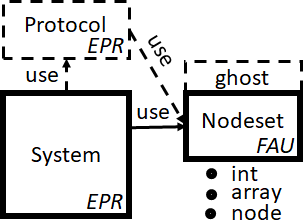
\includegraphics[scale=0.4]{fig-toy-modules-3}
%\end{minipage}
\caption{\label{fig:toy-c}Toy Leader Election pseudocode.}
\end{figure}
